
\documentclass[10pt,openany,a4paper]{article}
\usepackage{tikz, pgfplots, tkz-euclide,calc}
\usetikzlibrary{patterns,shapes.arrows,calc}
\usepackage{fancyhdr}
\usepackage{enumerate,enumitem}
\usepackage{cancel}
\usepackage{varwidth}

% TAMBAHKAN PACKAGE SENDIRI KALAU KURANG

\usepackage{geometry}
\geometry{
	left = 22mm,
	right = 22mm,
	top = 25mm,
	bottom = 25mm,
}
\usepackage{graphicx}
\usepackage{subcaption}
\usepackage{soul}
\usepackage{hyperref}
\usepackage{float}
\usepackage{setspace}
\usepackage{afterpage}
\usepackage{xcolor}
\usepackage[nosectionbib]{apacite}
\usepackage{lmodern}
\usepackage{mathtools}
\usepackage{upgreek}
\usepackage{siunitx}
% \usepackage{fontawesome5}
\usepackage{fontawesome6}
\usepackage{physics}
\usepackage{pdfpages}
\usepackage{hyperref}
\renewcommand{\baselinestretch}{1.3}
\usepackage{multicol}
\usepackage{hyperref,ragged2e,amsmath,multicol,gensymb,setspace,
fancyhdr,amsfonts,tikz,pgfplots,nccmath,enumerate,verbatim,amsthm,physics}
\usepgfplotslibrary{polar,fillbetween}
% Disable tikz externalization to avoid requiring -shell-escape
\usepgfplotslibrary{external}
\tikzexternalize[prefix=tikz/]
\tikzset{reuse path/.code={\pgfsyssoftpath@setcurrentpath{#1}}}
\usetikzlibrary{shapes.geometric,arrows}
\newcommand\mylog[1]{\mathop{{}^{#1}\mathrm{log}}}
\pgfplotsset{compat=1.15}
\pgfplotsset{my style/.append style={axis x line=middle, axis y line=
middle, xlabel={$x$}, ylabel={$y$}, axis equal }}
\usepackage{etoolbox}
% remove stray \makeatother
\newtheorem{defn}{Definisi}[section]
\newtheorem{teo}[defn]{Teorema}
\newtheorem{thm}{Teorema}[section]
\newtheorem{lemma}{Lemma}
\newtheorem{lemmas}[defn]{Lemma}
\newtheorem{cor}[defn]{Akibat}
\newtheorem{asumsi}[defn]{Asumsi}
\theoremstyle{definition}
\newtheorem{con}{Contoh}[section]
\theoremstyle{definition}
\theoremstyle{plain}
\newtheorem{prop}{Proposisi}[section]
\renewcommand{\proofname}{Bukti}
\renewcommand{\thethm}{\arabic{chapter}.\arabic{thm}}

\newcommand{\normlp}[1]{\left\|#1\right\|_{L^p_{\lambda}(0,T;H)}}% Fungsi norm (||x||)
\newcommand{\R}{\mathbb{R}}
\renewcommand{\natural}{\mathbb{N}}
\newcommand{\Xpl}{X^R_{p,\lambda}}
\newcommand{\Xpls}{X^R_{p,\lambda^*}}
\newcommand{\qpl}{q^R_{p,\lambda}}
\newcommand{\qpls}{q^R_{p,\lambda^*}}
\pagestyle{fancy}
\fancyhf{}
\lhead{Halaman \thepage}
% \cfoot{\faXTwitter\ \href{https://x.com/ahmadzakiyudin_/}{@ahmadzakiyudin\_} | \faInstagram\ \href{https://instagram.com/ahmadzakiyudin_/}{@ahmadzakiyudin\_} | \faTiktok\ \href{https://tiktok.com/@ahmathz/}{@ahmathz}}
% \rhead{Pembahasan Soal ETS \\ Kalkulus 1 ITS 2025/2026}
\hypersetup{
    colorlinks=true,
    linkcolor=blue,
    filecolor=blue,      
    urlcolor=blue,
}
\newenvironment{jawab}[2][tes]{
% \fbox{\begin{minipage}{14.65cm}
\textbf{Kata kunci materi:} #1.\\
\textbf{Penyelesaian:} #2
% \end{minipage}}
}{}

\newenvironment{jawab2}[2][tes]{
\fbox{\begin{minipage}{14.65cm}
 #2
\end{minipage}}}{}

\newenvironment{jawaban}[2][tes]{
\colorlet{oldcolor}{.}
        \color{red}
        \setlength{\fboxrule}{1pt}\boxed{\color{oldcolor}#2}\color{oldcolor}.
}{}

\newenvironment{jawaban2}[2][tes]{
\colorlet{oldcolor}{.}
        \color{red}
        \setlength{\fboxrule}{1pt}\fbox{\color{oldcolor}#2}\color{oldcolor}.
}{}

\newenvironment{penting}[2][tes]{
\colorlet{oldcolor}{.}
\color{blue}
\fbox{\color{oldcolor}#2}\color{oldcolor}
}{}

\begin{document}
% \begin{titlepage}
%     \vspace*{\fill}
%     \begin{center}
%       \Huge {PEMBAHASAN SOAL EAS \\ KALKULUS II \\ TAHUN 2024/2025}\\[0.4 cm]
%       \huge {Ahmad Hisbu Zakiyudin}\\[0.2 cm]
%       \Large {(\href{https://instagram.com/ahmadzakiyudin_/}{@ahmadzakiyudin\_})}
%     \end{center}
%     \vspace*{\fill}
%   \end{titlepage}
% !TEX root = ../../BookTemplate.tex
%%%%%%%%%%%%%%%%%%%%%%%%%%%%%%%%%%%%%%%%%%%%%%%%%%%%%%%%%%%%%%%%%%%%%%%%%%%%%%%%%%
% \begin{titlepage}
%     \raggedleft	
% 	\hspace{.025\textwidth}
% 	\parbox[b]{\textwidth}{
%     \vspace{1.5cm}
% 		{\Huge\bfseries Pembahasan Soal EAS}                \\[20pt]
% 		{\huge\textit\ Kalkulus II}\\ \\[10pt]
%         {\Large\textsc{Tahun 2024/2025}}}
% \vfill
% \rule{1pt}{.14\textheight}
% \hspace{.025\textwidth}
%     \raisebox{10pt}{\parbox[b]{.95\textwidth}{ 
%         {\Large\textsc{Ahmad Hisbu Zakiyudin}}              \\[10pt]
%         \large{\href{https://instagram.com/ahmadzakiyudin_/}{@ahmadzakiyudin\_}}               \\[25pt]
%         {\large 5 Juni 2026}}}
% \end{titlepage}
\begin{titlepage}
	\centering % Center everything on the title page
	% \scshape % Use small caps for all text on the title page
	\vspace*{1.5\baselineskip} % White space at the top of the page
% ===================
%	Title Section 	
% ===================

	\rule{13cm}{1.6pt}\vspace*{-\baselineskip}\vspace*{2pt} % Thick horizontal rule
	\rule{13cm}{0.4pt} % Thin horizontal rule
	
		\vspace{0.75\baselineskip} % Whitespace above the title
% ========== Title ===============	
	{	\Huge Soal Tryout ETS\\ 
			\vspace{4mm}
		Kalkulus 1 \\ \vspace{2mm} \huge{Tahun 2026/2027}\\	}
% ======================================
		\vspace{0.75\baselineskip} % Whitespace below the title
	\rule{13cm}{0.4pt}\vspace*{-\baselineskip}\vspace{3.2pt} % Thin horizontal rule
	\rule{13cm}{1.6pt} % Thick horizontal rule
	
		\vspace{1.75\baselineskip} % Whitespace after the title block
% =================
%	Information	
% =================
{\large Oleh: Ahmad Hisbu Zakiyudin}
	% {\large Oleh: Ahmad Hisbu Zakiyudin \\
	% 	\vspace*{1.2\baselineskip}
	% \href{https://instagram.com/ahmadzakiyudin_/}{@ahmadzakiyudin\_}} \\
	\vfill
	\vspace{1mm}
\huge{Selamat Belajar!}
\end{titlepage}
\makeatletter
\setlength\fboxsep{3pt}
% ensure enough header height for fancyhdr
\setlength{\headheight}{24pt}
% Kop tiap kelompok: #1 kelompok, #2 kelas, #3 departemen, #4 jadwal kuliah, #5 sesi
\newcommand{\kopsoal}[5]{%
 \begin{center}
	{\underline{\textbf{\MakeUppercase{Tryout ETS Kalkulus 1 Tahun 2026/2027}}}}
    \end{center}

    \begin{center}
	\begin{tabular}{lcl}
		Mata kuliah/SKS & : & Kalkulus 1 ( SM234101 ) / 3 SKS\\
		Kelompok & : & #1\\
		Kelas & : & #2\\
		Departemen & : & #3\\
		Jadwal kuliah & : & #4\\
		Sesi & : & #5\\
		Waktu & : & 100 menit\\
		Sifat & : & Tertutup\\
  ~
	\end{tabular}

    \noindent\rule{\textwidth}{2.pt}
        \end{center}}

% Kop kelompok IUP (bahasa Inggris): #1 kelompok, #2 kelas, #3 departemen, #4 jadwal kuliah, #5 sesi
\newcommand{\kopsoaliup}[5]{%
 \begin{center}
	{\underline{\textbf{\MakeUppercase{Tryout ETS Kalkulus 1 Tahun 2026/2027}}}}
    \end{center}

    \begin{center}
	\begin{tabular}{lcl}
		Course / Credit & : & Kalkulus 1 ( SM234101 ) / 3 SKS\\
		Group & : & #1\\
		Class & : & #2\\
		Department & : & #3\\
		Lecture schedule & : & #4\\
		Session & : & #5\\
		Time & : & 100 minutes\\
		Type & : & Closed\\
  ~
	\end{tabular}

    \noindent\rule{\textwidth}{2.pt}
        \end{center}}

% Kop tryout Matematika 2 SKS: #1 kelompok, #2 kelas, #3 departemen, #4 jadwal kuliah, #5 sesi
\newcommand{\kopsoalmat}[5]{%
 \begin{center}
	{\underline{\textbf{\MakeUppercase{Tryout ETS Matematika Tahun 2026/2027}}}}
    \end{center}

    \begin{center}
	\begin{tabular}{lcl}
		Mata kuliah/SKS & : & Matematika ( SM234152 ) / 2 SKS\\
		Kelompok & : & #1\\
		Kelas & : & #2\\
		Departemen & : & #3\\
		Jadwal kuliah & : & #4\\
		Sesi & : & #5\\
		Waktu & : & 100 menit\\
		Sifat & : & Tertutup\\
  ~
	\end{tabular}

    \noindent\rule{\textwidth}{2.pt}
        \end{center}}

% Kop tryout Matematika 2 SKS IUP (bahasa Inggris)
\newcommand{\kopsoalmatiup}[5]{%
 \begin{center}
	{\underline{\textbf{\MakeUppercase{Tryout ETS Matematika Tahun 2026/2027}}}}
    \end{center}

    \begin{center}
	\begin{tabular}{lcl}
		Course / Credit & : & Matematika ( SM234152 ) / 2 SKS\\
		Group & : & #1\\
		Class & : & #2\\
		Department & : & #3\\
		Lecture schedule & : & #4\\
		Session & : & #5\\
		Time & : & 100 minutes\\
		Type & : & Closed\\
  ~
	\end{tabular}

    \noindent\rule{\textwidth}{2.pt}
        \end{center}}

%%%%%%%%%%%%%%%%%%%%%%%%%%%%%%%%%%%%%%%%%%%%%%%%%%%%%%%%%%%%%%%%%%%%%%%%%%%%%%
% Kal-5 | acuan: ETS 25-26 Senin 07.00, ETS 24-25 Kamis 11.00, ETS 23-24 Selasa 07.00/09.00
\kopsoal{Kal-5}{22-27}{T. Fisika, T. Material dan Metalurgi, Rkp}{Senin, Rabu; 07.00-09.30}{1}
\begin{enumerate}
    \item Dapatkan himpunan penyelesaian pertidaksamaan
    \begin{align*}
        3\leq\frac{x^2+2}{x}<x+2
    \end{align*}

    \item Diberikan fungsi $f(x)=\dfrac{1}{x+2}$ dan $g(x)=3-\sqrt{x}$.
    \begin{enumerate}
        \item Tentukan domain dari fungsi $f$ dan $g$.
        \item Dapatkan fungsi $(f\circ g)(x)$ beserta domainnya.
    \end{enumerate}

    \item Diberikan suatu fungsi $f(x)=1+\sqrt{4-x^2}$ dengan domain $f$ adalah $[a,2]$.
    \begin{enumerate}
        \item Tentukan nilai terkecil $a$ agar $f^{-1}(x)$ ada.
        \item Dapatkan $f^{-1}(x)$.
        \item Dapatkan domain dan range dari $f^{-1}(x)$.
    \end{enumerate}

    \item Diberikan fungsi $f(x)=\begin{cases}
        \dfrac{x^3-27}{3x-9}, & x\neq 3\\
        k, & x=3
    \end{cases}$.
    \begin{enumerate}
        \item Tentukan nilai $k$ sehingga $f(x)$ kontinu di $x=3$.
        \item Berdasarkan hasil dari (a), nyatakan $f(x)$ sebagai polinomial.
    \end{enumerate}

    \item Diberikan fungsi implisit $x^2+2y^2-3xy+2x-y=3$.
    \begin{enumerate}
        \item Tentukan $\dfrac{dy}{dx}$ di titik $(2,1)$.
        \item Dapatkan persamaan garis singgung kurva di titik tersebut.
    \end{enumerate}
\end{enumerate}

\newpage

%%%%%%%%%%%%%%%%%%%%%%%%%%%%%%%%%%%%%%%%%%%%%%%%%%%%%%%%%%%%%%%%%%%%%%%%%%%%%%
% Kal-6 | acuan: ETS 25-26 Senin 07.00, ETS 24-25 Rabu 07.00, ETS 23-24 Selasa 11.00
\kopsoal{Kal-6}{28-31}{T. Perkapalan, T. Transportasi Laut, T. Bangunan Lepas Pantai}{Senin, Rabu; 07.00-09.30}{1}
\begin{enumerate}
    \item Diketahui garis $g_1: y=-2x+8$ dan garis $g_2: y=x+2$.
    \begin{enumerate}
        \item Tentukan titik potong kedua garis $g_1$ dan $g_2$.
        \item Tentukan titik potong $g_1$ dan $g_2$ masing-masing dengan garis $x=4$.
        \item Gambarkan sketsa ketiga garis $g_1$, $g_2$, dan garis $x=4$. Hitung luas segitiga yang dibentuk ketiga garis tersebut.
    \end{enumerate}

    \item Diberikan $f(x)=\dfrac{1}{x^2-9}$ dan $g(x)=\sqrt{x+2}$.
    \begin{enumerate}
        \item Dapatkan domain $f(x)$ dan $g(x)$.
        \item Dapatkan $(f\circ g)(x)$ dan domain $(f\circ g)(x)$.
    \end{enumerate}

    \item Diberikan fungsi sebagai berikut:
    \begin{align*}
        f(x)=\frac{2}{x-1};\quad \text{dan}\quad g(x)=\frac{x+2}{x}
    \end{align*}
    \begin{enumerate}
        \item Tentukan domain dan range dari masing-masing fungsi tersebut.
        \item Apakah kedua fungsi tersebut saling invers? Jelaskan alasannya.
    \end{enumerate}

    \item Dapatkan nilai $k$ sedemikian sehingga fungsi:
    \begin{align*}
        f(x)=\begin{cases}
            kx^2-1, & x<2\\
            3x+k, & x\geq 2
        \end{cases}
    \end{align*}
    kontinu di $x=2$.

    \item Dapatkan $f'(x)$ untuk $x>\frac{1}{2}$, dimana $f(x)=\sqrt{\dfrac{(2x-1)^3}{x}}$.
\end{enumerate}

\newpage

%%%%%%%%%%%%%%%%%%%%%%%%%%%%%%%%%%%%%%%%%%%%%%%%%%%%%%%%%%%%%%%%%%%%%%%%%%%%%%
% Kal-iup-1 | acuan: ETS 25-26 IUP Monday 09.00 (Kal-iup-1 25-26 = T. Kimia, T. Lingkungan, T. Elektro), reguler 24-25 Kamis 07.00/09.00/11.00, 23-24 Senin 11.00 & Selasa 07.00/09.00/13.30/15.30
\kopsoaliup{Kal-iup-1}{61, 68}{Chemical, Environmental, Electrical Engineering}{Monday, Wednesday; 07.00-09.30}{1}
\begin{enumerate}
    \item Solve the following inequality.
    \begin{align*}
        \frac{x^2-2x-8}{x^2-4x+3}\geq 0.
    \end{align*}

    \item Given a function $f(x)=3-\sqrt{x}$ and $g(x)=\dfrac{1}{x+1}$. Determine:
    \begin{enumerate}
        \item[a)] The domain of function $f$ and $g$;
        \item[b)] Function $(f\circ g)(x)$ and its domain.
    \end{enumerate}

    \item Write the derivative formula of $\dfrac{f}{g}$, that is $\dfrac{d}{dx}\left(\dfrac{f(x)}{g(x)}\right)$.\\
    Then, find the derivative of $\dfrac{f}{g}$ given that $f(x)=x^2+4x-5$ and $g(x)=x+2$ for $x\neq -2$.

    \item Given $f(x)=\begin{cases}
        \dfrac{x^3+27}{x+3}, & x\neq -3\\
        3k, & x=-3
    \end{cases}$.
    \begin{enumerate}
        \item[a.] Determine $k$ such that $f(x)$ is continuous at $x=-3$.
        \item[b.] Based on the result of a), rewrite $f(x)$ as a polynomial.
    \end{enumerate}

    \item Sketch the base curve $x=y^2$. Based on that base curve, use translation to sketch the curve $x=y^2-2y-3$. (Explain the process).
\end{enumerate}

\newpage

%%%%%%%%%%%%%%%%%%%%%%%%%%%%%%%%%%%%%%%%%%%%%%%%%%%%%%%%%%%%%%%%%%%%%%%%%%%%%%
% Kal-iup-4 | acuan: ETS 25-26 IUP Monday 09.00 (Kal-iup-4 25-26 = Statistika, T. Sistem Perkapalan, T. Informatika), reguler 24-25 Rabu 07.00/Kamis 09.00/Kamis 13.30, 23-24 Senin 07.00/09.00 & Selasa 11.00/13.30/15.30
\kopsoaliup{Kal-iup-4}{65, 66, 67}{Statistics, Marine Engineering (JD), Informatics}{Monday, Wednesday; 07.00-09.30}{1}
\begin{enumerate}
    \item Solve the following inequality.
    \begin{align*}
        \frac{x^2+2x-15}{x^2-x-2}\geq 0.
    \end{align*}

    \item Given a function $f(x)=1-\sqrt{x}$ and $g(x)=\dfrac{4}{x-2}$. Determine:
    \begin{enumerate}
        \item[a)] The domain of function $f$ and $g$;
        \item[b)] Function $(f\circ g)(x)$ and its domain.
    \end{enumerate}

    \item Write the derivative formula of $\dfrac{f}{g}$, that is $\dfrac{d}{dx}\left(\dfrac{f(x)}{g(x)}\right)$.\\
    Then, find the derivative of $\dfrac{f}{g}$ given that $f(x)=3x^2-5x-2$ and $g(x)=x-2$ for $x\neq 2$.

    \item Given $f(x)=\begin{cases}
        \dfrac{x^3-1}{2x-2}, & x\neq 1\\
        3k, & x=1
    \end{cases}$.
    \begin{enumerate}
        \item[a.] Determine $k$ such that $f(x)$ is continuous at $x=1$.
        \item[b.] Based on the result of a), rewrite $f(x)$ as a polynomial.
    \end{enumerate}

    \item Sketch the base curve $x=y^2$. Based on that base curve, use translation to sketch the curve $x=y^2+6y+5$. (Explain the process).
\end{enumerate}

\newpage

%%%%%%%%%%%%%%%%%%%%%%%%%%%%%%%%%%%%%%%%%%%%%%%%%%%%%%%%%%%%%%%%%%%%%%%%%%%%%%
% Kal-9 | acuan: ETS 25-26 Senin 07.00, ETS 24-25 Rabu 07.00 & Kamis 09.00, ETS 23-24 Selasa 11.00 & Selasa 13.30 & 15.30
\kopsoal{Kal-9}{44-48}{T. Sistem Perkapalan, T. Kelautan, T. Komputer}{Senin, Rabu; 12.30-15.00}{3}
\begin{enumerate}
    \item Dapatkan penyelesaian dari $|x+1|=|2x-3|+1$.

    \item Diberikan titik $A(1,-2)$, $B(-1,3)$ dan $C(3,1)$.
    \begin{enumerate}
        \item Dapatkan persamaan garis yang melalui titik $A$ dan sejajar dengan garis yang melalui $B$ dan $C$.
        \item Dapatkan persamaan garis yang melalui titik $A$ dan tegak lurus dengan garis yang melalui $B$ dan $C$.
    \end{enumerate}

    \item Diberikan $f(x)=\sqrt[3]{x+2},\ x\geq -2$.
    \begin{enumerate}
        \item Dapatkan $f^{-1}(x)$ beserta domainnya.
        \item Sketsa $f(x)$ dan $f^{-1}(x)$ pada satu bidang koordinat.
    \end{enumerate}

    \item Hitunglah $\displaystyle\lim_{y\to-\infty}\frac{3-2y}{\sqrt{5+9y^2}}$.

    \item Dapatkan persamaan garis singgung kurva $x^2+y+\dfrac{2y}{x}=\sqrt{x}+3$ di titik $(1,1)$.
\end{enumerate}

\newpage

%%%%%%%%%%%%%%%%%%%%%%%%%%%%%%%%%%%%%%%%%%%%%%%%%%%%%%%%%%%%%%%%%%%%%%%%%%%%%%
% Kal-11 | acuan: ETS 25-26 Senin 13.30, ETS 24-25 Kamis 13.30 & Kamis 09.00, ETS 23-24 Senin 07.00/09.00 & Selasa 13.30 & 15.30
\kopsoal{Kal-11}{51-54}{Biologi, Bioteknologi, Teknologi Informasi}{Senin, Rabu; 12.30-15.00}{3}
\begin{enumerate}
    \item \begin{enumerate}
        \item Definisikan $|x-1|$.
        \item Berdasarkan point (a) tersebut, tentukan semua nilai $x$ yang memenuhi pertidaksamaan
        \begin{align*}
            |x-1|\leq 5-2x.
        \end{align*}
    \end{enumerate}

    \item \begin{enumerate}
        \item Tentukan jarak titik $(-3,4)$ dan $(5,-2)$.
        \item Tentukan persamaan lingkaran yang diameternya adalah ruas garis dari titik $(-3,4)$ ke $(5,-2)$.
    \end{enumerate}

    \item Diberikan fungsi $f(x)=-\sqrt{|x^2-9|}$ dan $g(x)=\dfrac{1}{x^2-4}$.
    \begin{enumerate}
        \item Dapatkan domain $f$ dan $g$.
        \item Dapatkan $(g\circ f)(x)$ beserta domainnya.
    \end{enumerate}

    \item Diberikan $f(x)=\begin{cases}
        k^2(x+1), & x\leq 1\\
        (3-k)x, & x>1
    \end{cases}$.\\
    Tentukan semua nilai $k$ yang memenuhi agar $\displaystyle\lim_{x\to 1}f(x)$ ada.

    \item Diketahui kurva $x^3+xy-y^2=1$.
    \begin{enumerate}
        \item Dapatkan $\dfrac{dy}{dx}$ dengan menggunakan turunan fungsi implisit.
        \item Dari (a) dapatkan persamaan garis singgung pada kurva tersebut di titik $(1,1)$.
    \end{enumerate}
\end{enumerate}

\newpage

%%%%%%%%%%%%%%%%%%%%%%%%%%%%%%%%%%%%%%%%%%%%%%%%%%%%%%%%%%%%%%%%%%%%%%%%%%%%%%
% Kal-12 | acuan: ETS 25-26 Senin 11.00, ETS 24-25 Kamis 13.30 & Kamis 09.00, ETS 23-24 Senin 07.00/09.00 & Selasa 13.30 & 15.30
\kopsoal{Kal-12}{55-60}{Aktuaria, Teknik Informatika, RPL, RKA}{Senin, Rabu; 12.30-15.00}{3}
\begin{enumerate}
    \item \begin{enumerate}
        \item Nyatakan pernyataan $\sqrt{(3x+2)^2}$ dalam bentuk nilai mutlak.
        \item Dapatkan semua nilai $x$ yang memenuhi persamaan $\sqrt{(3x+2)^2}=3x+2$.
    \end{enumerate}

    \item Diberikan fungsi $f(x)=\sqrt{x+3}$.
    \begin{enumerate}
        \item Tentukan domain dan range dari fungsi $f(x)$.
        \item Tentukan $f^{-1}(x)$, domain dan range dari $f^{-1}(x)$.
    \end{enumerate}

    \item Diberikan persamaan separuh lingkaran
    \begin{align*}
        x=-2-\sqrt{-y^2+4y+12}.
    \end{align*}
    \begin{enumerate}
        \item Dapatkan pusat dan jari-jari lingkaran.
        \item Sketsa grafiknya.
    \end{enumerate}

    \item Diberikan fungsi $f(x)=\dfrac{9-x^2}{3-|x|}$.
    \begin{enumerate}
        \item Nyatakan fungsi $f(x)$ dalam bentuk fungsi sepotong-sepotong.
        \item Selidiki apakah $f(x)$ memiliki titik diskontinu.
        \item Jika memiliki titik diskontinu, apakah titik diskontinu dapat dihilangkan?
    \end{enumerate}

    \item Diketahui fungsi $f(x)=\left(x^2-\dfrac{4}{x}\right)^{3/2}$. Dapatkan $f'(2)$.
\end{enumerate}

\newpage

%%%%%%%%%%%%%%%%%%%%%%%%%%%%%%%%%%%%%%%%%%%%%%%%%%%%%%%%%%%%%%%%%%%%%%%%%%%%%%
% Kal-7 | acuan: ETS 25-26 Senin 13.30, ETS 24-25 Kamis 07.00, ETS 23-24 Senin 11.00
\kopsoal{Kal-7}{32-37}{T. Sipil, T. Geomatika, T. Geofisika, T. Pertambangan}{Senin, Rabu; 15.30-17.10}{4}
\begin{enumerate}
    \item \begin{enumerate}
        \item Definisikan $|x+2|$.
        \item Berdasarkan point (a) tersebut, tentukan semua nilai $x$ yang memenuhi pertidaksamaan
        \begin{align*}
            |x+2|\leq 3x-2.
        \end{align*}
    \end{enumerate}

    \item \begin{enumerate}
        \item Tentukan jarak titik $(-2,1)$ dan $(4,9)$.
        \item Tentukan persamaan lingkaran yang diameternya adalah ruas garis dari titik $(-2,1)$ ke $(4,9)$.
    \end{enumerate}

    \item Diberikan suatu fungsi $f(x)=3-\sqrt{9-x^2}$ dengan domain $f$ adalah $[a,3]$.
    \begin{enumerate}
        \item Tentukan nilai terkecil $a$ agar $f^{-1}(x)$ ada.
        \item Dapatkan $f^{-1}(x)$.
        \item Sketsa grafik $f(x)$ dan $f^{-1}(x)$ pada satu bidang koordinat.
    \end{enumerate}

    \item Hitunglah $\displaystyle\lim_{x\to-\infty}\frac{\sqrt{9x^2+1}}{2x-5}$.

    \item Diketahui kurva $x^2y+3x-2y^2=-3$.
    \begin{enumerate}
        \item Dapatkan $\dfrac{dy}{dx}$ dengan menggunakan turunan fungsi implisit.
        \item Dari (a) dapatkan persamaan garis singgung pada kurva tersebut di titik $(1,2)$.
    \end{enumerate}
\end{enumerate}

\newpage

%%%%%%%%%%%%%%%%%%%%%%%%%%%%%%%%%%%%%%%%%%%%%%%%%%%%%%%%%%%%%%%%%%%%%%%%%%%%%%
% Kal-8 | acuan: ETS 25-26 Senin 13.30, ETS 24-25 Kamis 13.30, ETS 23-24 Senin 07.00/09.00
\kopsoal{Kal-8}{38-43}{Matematika, Statistika, Sains Data}{Senin, Rabu; 15.30-17.10}{4}
\begin{enumerate}
    \item Diberikan tiga titik koordinat $A(0,1)$, $B(4,4)$ dan $C(1,6)$.
    \begin{enumerate}
        \item Dapatkan persamaan garis lurus $\ell$ yang melalui titik $A$ dan $B$.
        \item Dapatkan persamaan garis lurus $k$ yang melalui titik $C$ dan tegak lurus dengan garis $\ell$.
        \item Dapatkan jarak titik $C$ ke garis lurus $\ell$.
    \end{enumerate}

    \item Diberikan fungsi $f(x)=\begin{cases}
        2x+1, & x<1\\
        (x-2)^2, & x\geq 1
    \end{cases}$.
    \begin{enumerate}
        \item Dapatkan $f(1)$, $f(-3)$, dan $f(-x^2)$.
        \item Dapatkan domain dan range dari $f(x)$.
        \item Sketsa grafik dari $f(x)$.
    \end{enumerate}

    \item Diberikan fungsi $f(x)=\sqrt{4x-x^2},\ 0\leq x\leq 2$.
    \begin{enumerate}
        \item Tentukan $f^{-1}(x)$ beserta domainnya.
        \item Gambarkan grafik $f(x)$ dan $f^{-1}(x)$ dalam satu bidang koordinat.
    \end{enumerate}

    \item Diberikan $f(x)=\dfrac{x^3+8}{x+2}$.
    \begin{enumerate}
        \item Tentukan $\displaystyle\lim_{x\to -2}f(x)$.
        \item Buatlah sketsa grafik $y=f(x)$.
    \end{enumerate}

    \item Diketahui garis singgung pada kurva $x^2-xy+y^2=12$ di titik $(a,b)$ sejajar dengan sumbu-$x$. Tentukan semua titik $(a,b)$ dan persamaan garis singgungnya.
\end{enumerate}

\newpage

%%%%%%%%%%%%%%%%%%%%%%%%%%%%%%%%%%%%%%%%%%%%%%%%%%%%%%%%%%%%%%%%%%%%%%%%%%%%%%
% Kal-iup-2 | acuan: ETS 25-26 IUP Tuesday 07.00 (Kal-iup-2 25-26 = T. Mesin, Teknik Sistem dan Industri, T. Material), reguler 24-25 Kamis 11.00, 23-24 Selasa 07.00/09.00
\kopsoaliup{Kal-iup-2}{62, 69}{Mechanical, Industrial, Materials \& Metallurgical Engineering}{Monday, Wednesday; 15.30-17.10}{4}
\begin{enumerate}
    \item Find the solution of the following inequality
    \begin{align*}
        \frac{x^2+x-6}{x^2-3x-4}\geq 0.
    \end{align*}

    \item \begin{enumerate}
        \item Find the gradient of the line $\ell$ which goes through $(0,0)$ and $(3,-4)$.
        \item If line $\ell$ is perpendicular with the line that tangent with a circle centered at $(0,0)$ and radius $5$, at $(3,-4)$, then find the aforementioned tangent line equation and sketch the graph.
    \end{enumerate}

    \item Write the derivative formula of $fg$ that is $\dfrac{d}{dx}(f(x)g(x))$\\
    Then, find the derivative of $fg$, given that $f(x)=2x^3-x$ and $g(x)=4-x^2$.

    \item Calculate $\displaystyle\lim_{x\to 2}\frac{\sqrt{4x+1}-3}{x-2}$.

    \item Given a function $f(x)=\dfrac{1}{x+2}$ and $g(x)=x^2$.
    \begin{enumerate}
        \item Find $(f\circ g)(x)$.
        \item Given $(p\circ g)(x)=x^2+5$, then find $p(x)$.
    \end{enumerate}
\end{enumerate}

\newpage

%%%%%%%%%%%%%%%%%%%%%%%%%%%%%%%%%%%%%%%%%%%%%%%%%%%%%%%%%%%%%%%%%%%%%%%%%%%%%%
% Kal-3 | acuan: ETS 25-26 Selasa 15.30, ETS 24-25 Kamis 13.30 & Kamis 09.00, ETS 23-24 Senin 07.00/09.00 & Selasa 13.30 & 15.30
\kopsoal{Kal-3}{13-16}{Kimia, Saik, Telkom}{Selasa, Kamis; 07.00-09.30}{6}
\begin{enumerate}
    \item Dapatkan penyelesaian dari pertidaksamaan
    \begin{align*}
        1\leq x^2-3\leq 13.
    \end{align*}

    \item Tentukan domain dari fungsi $(f\circ g)(x)$ jika diketahui fungsi $g(x)=3x-1$ dengan $0\leq x<2$ dan fungsi $f$ terdefinisi pada interval $1\leq x<4$.

    \item Gunakan grafik dasar $x=y^2$ dan sifat pergeseran/translasi untuk menggambar parabola $x=y^2-4y+1$.

    \item Diberikan $f(x)=\begin{cases}
        k^2(x-1), & x\leq 2\\
        k(x+1), & x>2
    \end{cases}$.\\
    Tentukan semua nilai $k$ yang memenuhi agar $\displaystyle\lim_{x\to 2}f(x)$ ada.

    \item Diketahui garis singgung pada kurva $x^2+xy+y^2=3$ di titik $(a,b)$ sejajar dengan garis $y=-x$. Tentukan semua titik $(a,b)$ dan persamaan garis singgungnya.
\end{enumerate}

\newpage

%%%%%%%%%%%%%%%%%%%%%%%%%%%%%%%%%%%%%%%%%%%%%%%%%%%%%%%%%%%%%%%%%%%%%%%%%%%%%%
% Kal-4 | acuan: ETS 25-26 Selasa 15.30, ETS 24-25 Kamis 11.00, ETS 23-24 Selasa 07.00/09.00
\kopsoal{Kal-4}{17-21}{T. Mesin, Teknik Sistem dan Industri}{Selasa, Kamis; 07.00-09.30}{6}
\begin{enumerate}
    \item Tentukan semua nilai $x$ yang memenuhi
    \begin{align*}
        1<\frac{1}{|x-3|}\leq 2.
    \end{align*}

    \item Diberikan $f(x)=\sqrt{16-x^2}$ dan $g(x)=\dfrac{1}{x^2-4}$.
    \begin{enumerate}
        \item Dapatkan domain $f(x)$ dan $g(x)$.
        \item Dapatkan $(g\circ f)(x)$ dan domain $(g\circ f)(x)$.
    \end{enumerate}

    \item Diberikan fungsi $f(x)=\left|\dfrac{x^2-4}{x+2}\right|$. Dapatkan titik $x$ di mana fungsi $f(x)$ diskontinu.\\
    Dapatkan nilai fungsi $f(x)$ pada titik tersebut agar menjadi kontinu dan sketsa grafik fungsi tersebut.

    \item Diberikan fungsi
    \begin{align*}
        f(x)=\begin{cases}
            \dfrac{x-16}{\sqrt{x}-4}, & x\neq 16\\
            7, & x=16
        \end{cases}.
    \end{align*}
    Selidiki kekontinuan $f(x)$ di $x=16$. Jika tidak kontinu, apakah diskontinuitasnya dapat dihilangkan? Jelaskan.

    \item Dapatkan $f''(x)$ dimana $f(x)=x^2+\left(3-\sqrt{x}\right)^{-1}$.
\end{enumerate}

\newpage

%%%%%%%%%%%%%%%%%%%%%%%%%%%%%%%%%%%%%%%%%%%%%%%%%%%%%%%%%%%%%%%%%%%%%%%%%%%%%%
% Kal-1 | acuan: ETS 25-26 Selasa 09.00, ETS 24-25 Kamis 11.00 & Kamis 13.30, ETS 23-24 Senin 07.00/09.00 & Selasa 07.00/09.00
\kopsoal{Kal-1}{1-6}{Fisika, T. Kimia, T. Pangan}{Selasa, Kamis; 12.30-15.00}{8}
\begin{enumerate}
    \item Selesaikan pertidaksamaan berikut
    \begin{align*}
        \frac{1}{x-3}\leq\frac{2}{x+1}.
    \end{align*}

    \item Diberikan fungsi $f(x)=\dfrac{1}{x-3}$ dan $g(x)=\sqrt{7-x}$. Tentukan:
    \begin{enumerate}
        \item Domain fungsi $f$ dan $g$.
        \item Fungsi $(f\circ g)(x)$ dan $\left(\dfrac{f}{g}\right)(x)$ beserta domainnya masing-masing.
    \end{enumerate}

    \item Diketahui $f(x)=\sqrt{9-x^2}$.
    \begin{enumerate}
        \item Tentukan domain $f(x)$.
        \item Apakah $f^{-1}(x)$ ada? Jelaskan alasannya.
        \item Jika tidak ada, definisikan domain $f(x)$ agar $f^{-1}(x)$ ada, kemudian dapatkan $f^{-1}(x)$ beserta domainnya.
    \end{enumerate}

    \item Diberikan fungsi
    \begin{align*}
        f(x)=\begin{cases}
            \dfrac{9-x}{3-\sqrt{x}}, & x\neq 9\\
            k, & x=9
        \end{cases},\quad \text{dengan } x\in[0,\infty).
    \end{align*}
    \begin{enumerate}
        \item Tentukan nilai $k$ sehingga $f(x)$ kontinu di $x=9$.
        \item Untuk nilai $k$ tersebut, nyatakan $f(x)$ tanpa menggunakan bentuk fungsi sepotong-sepotong.
    \end{enumerate}

    \item Dapatkan $f''(x)$ dimana $f(x)=3x+\left(2\sqrt{x}+1\right)^{-1}$.
\end{enumerate}

\newpage

%%%%%%%%%%%%%%%%%%%%%%%%%%%%%%%%%%%%%%%%%%%%%%%%%%%%%%%%%%%%%%%%%%%%%%%%%%%%%%
% Kal-2 | acuan: ETS 25-26 Selasa 09.00, ETS 24-25 Kamis 07.00 & Kamis 09.00, ETS 23-24 Senin 11.00 & Selasa 13.30 & 15.30
\kopsoal{Kal-2}{7-12}{T. Lingkungan, T. Elektro, T. Biomedik}{Selasa, Kamis; 12.30-15.00}{8}
\begin{enumerate}
    \item Diberikan garis $\ell$ melalui titik $(3,2)$ dan $(a,b)$ dengan kemiringan $2$, dan garis $k$ melalui titik $(0,-1)$ dan $(a,b)$ dengan kemiringan $-1$. Dapatkan nilai $a$ dan $b$.

    \item Gambarkan kurva dasar $y=\dfrac{1}{x}$. Berdasarkan kurva dasar tersebut, gunakan translasi (pergeseran) untuk menggambar kurva $y=\dfrac{1}{x+1}-2$ (Jelaskan ilustrasinya).

    \item Diberikan fungsi $f(x)=\sqrt[3]{x-1}+3$.
    \begin{enumerate}
        \item Dapatkan $f^{-1}(x)$.
        \item Dapatkan domain dan range dari $f^{-1}(x)$.
        \item Sketsa grafik dari $f(x)$ dan $f^{-1}(x)$ pada satu bidang koordinat.
    \end{enumerate}

    \item Hitunglah $\displaystyle\lim_{x\to-\infty}\frac{\sqrt{4x^2+3}}{2-x}$.

    \item Dapatkan persamaan garis singgung kurva $xy^2+2y-\sqrt{x}=2$ di titik $(1,1)$.
\end{enumerate}

\newpage

%%%%%%%%%%%%%%%%%%%%%%%%%%%%%%%%%%%%%%%%%%%%%%%%%%%%%%%%%%%%%%%%%%%%%%%%%%%%%%
% Kal-10 | acuan: ETS 25-26 Selasa 09.00, ETS 24-25 Kamis 07.00, ETS 23-24 Selasa 13.30 & 15.30
\kopsoal{Kal-10}{49-50}{Teknologi Kedokteran}{Selasa, Kamis; 12.30-15.00}{8}
\begin{enumerate}
    \item Dapatkan himpunan penyelesaian dari $\dfrac{2}{x+1}<\dfrac{1}{3-x}$.

    \item Diberikan fungsi $f(x)=\sqrt{2-x}$ dan $g(x)=\dfrac{1}{\sqrt{16-x^2}}$.
    \begin{enumerate}
        \item Dapatkan domain $f$ dan $g$.
        \item Dapatkan $(g\circ f)(x)$ beserta domainnya.
    \end{enumerate}

    \item Diberikan suatu fungsi $f(x)=1-\sqrt{6x-x^2}$ dengan domain $f$ adalah $[0,a]$.
    \begin{enumerate}
        \item Dapatkan nilai terbesar $a$ sehingga $f^{-1}(x)$ ada.
        \item Tentukan $f^{-1}(x)$.
        \item Gambarkan sketsa kurva $f(x)$ dan $f^{-1}(x)$ dalam satu bidang koordinat.
    \end{enumerate}

    \item Tunjukkan bahwa $f(x)=\begin{cases}
        x^2+1, & x\leq 1\\
        4x-2, & x>1
    \end{cases}$ adalah fungsi kontinu tetapi tidak dapat diturunkan di $x=1$.

    \item Diketahui kurva $xy^2+y^3=2x+8$.
    \begin{enumerate}
        \item Tentukan $\dfrac{dy}{dx}$.
        \item Dapatkan persamaan garis singgung kurva tersebut di titik $(0,2)$.
    \end{enumerate}
\end{enumerate}

\newpage

%%%%%%%%%%%%%%%%%%%%%%%%%%%%%%%%%%%%%%%%%%%%%%%%%%%%%%%%%%%%%%%%%%%%%%%%%%%%%%
% Kal-iup-3 | acuan: ETS 25-26 IUP Tuesday 07.00 (Kal-iup-3 25-26 = T. Sipil, T. Geomatika, T. Geofisika, T. Perkapalan, Perkapalan JD), reguler 24-25 Kamis 07.00 & Rabu 07.00, 23-24 Senin 11.00 & Selasa 11.00
\kopsoaliup{Kal-iup-3}{63, 64, 70}{Civil, Geomatics, Geophysical Engineering, Naval Architecture (JD)}{Tuesday, Thursday; 15.30-17.10}{9}
\begin{enumerate}
    \item Find the solution of the following inequality
    \begin{align*}
        \frac{x^2-5x+4}{x^2-x-6}\geq 0.
    \end{align*}

    \item \begin{enumerate}
        \item Find the gradient of the line $\ell$ which goes through $(0,0)$ and $(1,3)$.
        \item If line $\ell$ is perpendicular with the line that tangent with a circle centered at $(0,0)$ and radius $\sqrt{10}$, at $(1,3)$, then find the aforementioned tangent line equation and sketch the graph.
    \end{enumerate}

    \item Given $f(x)=x^3-1$.
    \begin{enumerate}
        \item Find $f^{-1}(x)$ and its domain.
        \item Sketch the graph of $f(x)$ and $f^{-1}(x)$ in the same coordinate plane.
    \end{enumerate}

    \item Calculate $\displaystyle\lim_{x\to-\infty}\frac{\sqrt{3x^2+1}}{x-2}$.

    \item Find the equation of the tangent line to the curve $x^2y^2+2xy=8y$ at the point $(2,1)$.
\end{enumerate}

\newpage

%%%%%%%%%%%%%%%%%%%%%%%%%%%%%%%%%%%%%%%%%%%%%%%%%%%%%%%%%%%%%%%%%%%%%%%%%%%%%%
% M2-14 | acuan: ETS Matematika (SM234152) 25-26 Jumat 07.00 (kelas 1-8), ETS Matematika 24-25 Senin 11.00 (kelas 1-7); soal M2 23-24 tidak tersedia
\kopsoalmat{M2-14}{1-7}{Sistem Informasi, Manajemen Bisnis, Studi Pembangunan, Bdigt, Skom}{Jum'at, 07.00-09.30}{11}
\begin{enumerate}
    \item Dapatkan himpunan penyelesaian dari $\dfrac{2}{x-2}\geq\dfrac{1}{x+1}$.

    \item Diketahui garis $l_1$ melalui titik $(-1,2)$ dan $(3,4)$.
    \begin{enumerate}
        \item Dapatkan persamaan garis $l_2$ yang melalui titik $(2,1)$ dan tegak lurus dengan garis $l_1$.
        \item Tentukan titik potong garis $l_1$ dan $l_2$.
    \end{enumerate}

    \item Diberikan SPL
    \begin{align*}
        x+2y-z &= 3\\
        2x-y+3z &= 6\\
        -x+y+2z &= 5
    \end{align*}
    \begin{enumerate}
        \item Nyatakan SPL tersebut dalam bentuk persamaan matriks $A\mathbf{x}=b$.
        \item Menggunakan eliminasi Gauss-Jordan, carilah solusi (jika ada) dari SPL tersebut.
    \end{enumerate}

    \item Diketahui fungsi $f(x)=x^2-4x-5$.
    \begin{enumerate}
        \item Dapatkan domain dan range dari $f(x)$.
        \item Sketsa grafik $f(x)$ beserta titik puncak dan titik potongnya dengan sumbu koordinat.
    \end{enumerate}

    \item Diberikan sistem persamaan fungsi permintaan dan penawaran (\textit{supply and demand})
    \begin{align*}
        3P &= -Q_d+150\\
        2P &= Q_s+25
    \end{align*}
    dengan $P,Q_d,Q_s$ masing-masing adalah harga, jumlah permintaan (\textit{demand}), dan jumlah penawaran (\textit{supply}).
    \begin{enumerate}
        \item Tentukan harga dan jumlah barang di titik equilibrium.
        \item Misalkan pemerintah memberikan pajak sebesar 5 untuk masing-masing barang. Tentukan persamaan fungsi penawaran setelah dikenakan pajak, titik equilibrium yang baru, dan pembagian pembayaran pajaknya.
        \item Gambarkan/sket kurva permintaan dan penawaran (sebelum dan sesudah pajak) beserta titik keseimbangannya.
    \end{enumerate}
\end{enumerate}

\newpage

%%%%%%%%%%%%%%%%%%%%%%%%%%%%%%%%%%%%%%%%%%%%%%%%%%%%%%%%%%%%%%%%%%%%%%%%%%%%%%
% M2-iup | acuan: ETS Matematika (SM234152) 25-26 Jumat 07.00 & 24-25 Senin 11.00 (kelas reguler, departemen sama); soal M2 IUP tahun sebelumnya tidak tersedia
\kopsoalmatiup{M2-iup}{8, 9}{Information Systems, Business Management}{Friday, 07.00-09.30}{11}
\begin{enumerate}
    \item Find the solution set of $\dfrac{3}{x+2}\leq\dfrac{1}{x-2}$.

    \item \begin{enumerate}
        \item Determine the value of $k$ such that the line $\ell_1: kx+2y=7$ is perpendicular to the line $\ell_2: 4x-6y=1$.
        \item Using the value of $k$ in (a), find the equation of the line passing through $(1,2)$ that is parallel to $\ell_1$.
    \end{enumerate}

    \item Given the system of linear equations
    \begin{align*}
        2x+y-z &= 3\\
        x-y+2z &= 1\\
        3x+2y+z &= 8
    \end{align*}
    \begin{enumerate}
        \item Write the system in the matrix equation form $A\mathbf{x}=b$.
        \item Using Gauss-Jordan elimination, find the solution (if any) of the system.
    \end{enumerate}

    \item Given the function $f(x)=-x^2+4x+5$.
    \begin{enumerate}
        \item Find the domain and range of $f(x)$.
        \item Sketch the graph of $f(x)$ including its vertex and its intersection points with the coordinate axes.
    \end{enumerate}

    \item Given the demand and supply functions
    \begin{align*}
        4P &= -Q_d+140\\
        3P &= Q_s+14
    \end{align*}
    where $P,Q_d,Q_s$ are the price, the quantity demanded, and the quantity supplied, respectively.
    \begin{enumerate}
        \item Find the equilibrium price and quantity.
        \item Suppose the government imposes a tax of 7 per unit. Find the supply function after tax, the new equilibrium point, and how the tax burden is shared between consumers and producers.
        \item Sketch the demand and supply curves (before and after tax) and the equilibrium points.
    \end{enumerate}
\end{enumerate}

\newpage
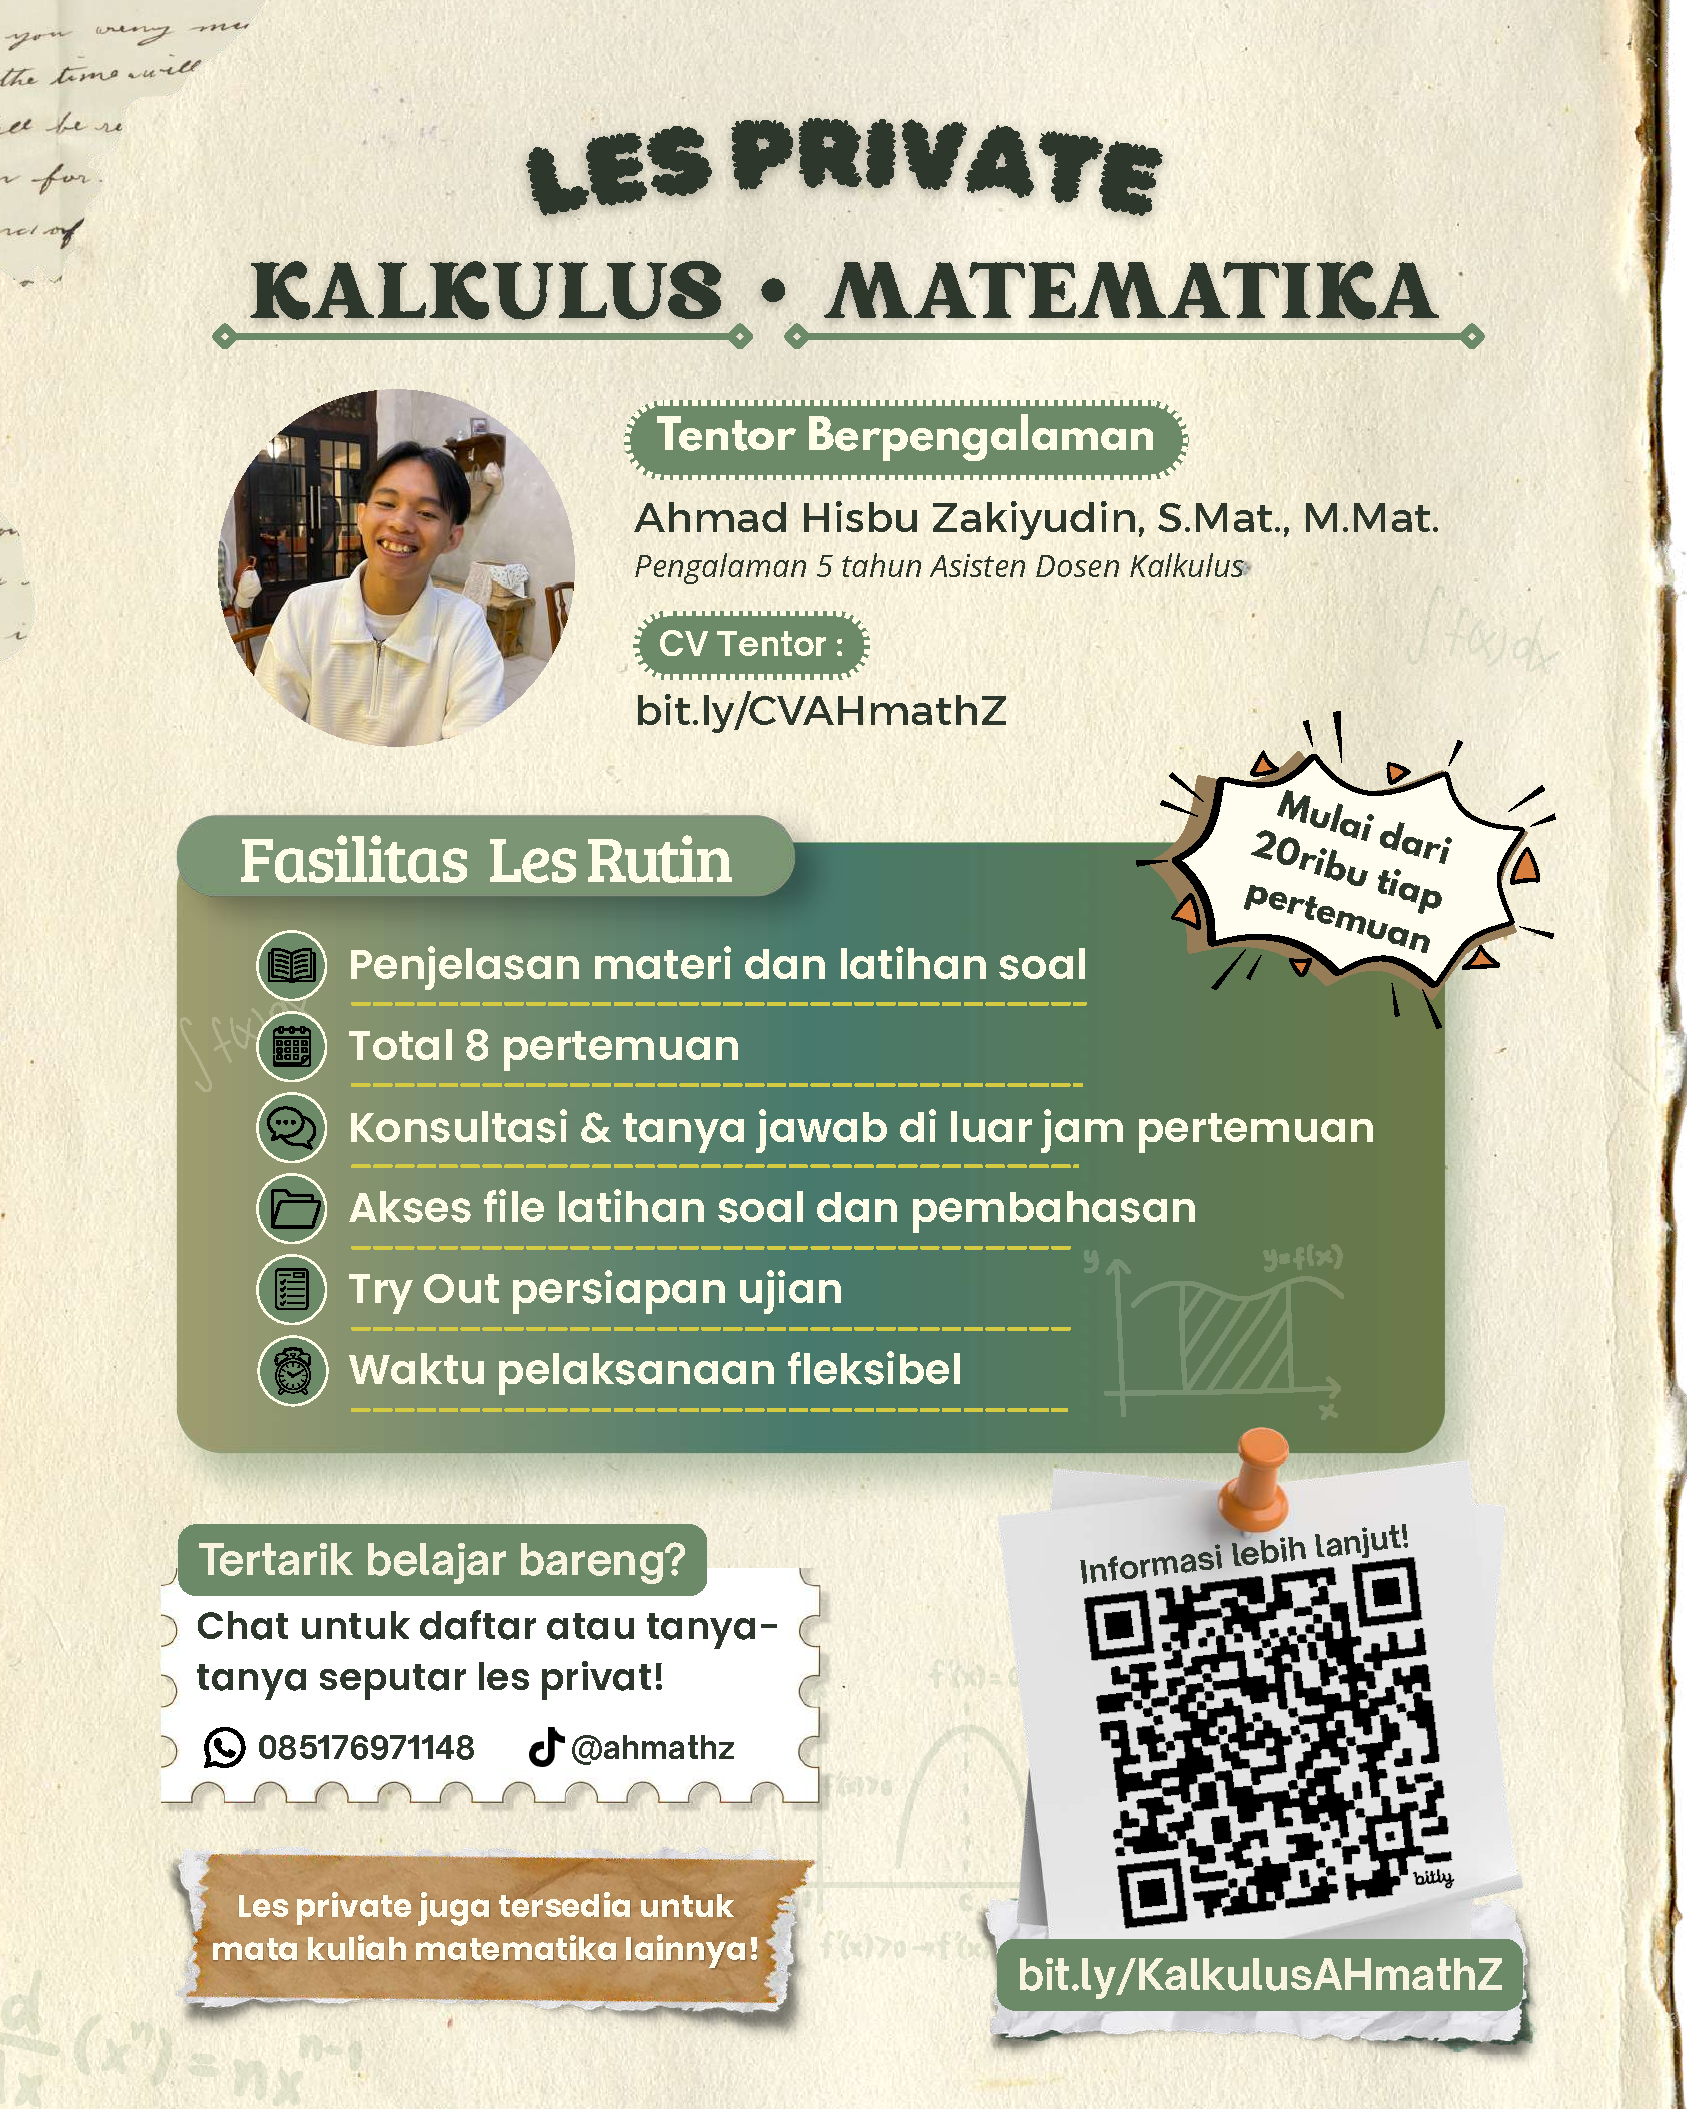
\includepdf[pages=-]{../ETS_Kalkulus_1_Th_2025-2026/les.pdf}

\end{document}
